%%%%%%%%%%%%%%%%%%%%
%
% $Autor: Wings $
% $Datum: 2020-02-24 14:29:03Z $
% $Pfad: komponenten/Bilderkennung/Produktspezifikation/CorelTPU/Ausarbeitung/Kapitel/Software.tex $
% $Version: 1791 $
%
%
%%%%%%%%%%%%%%%%%%%


%todo \url{https://www.kdnuggets.com/2017/09/tensorflow-tutorial-part-1.html}
%todo \url{https://www.kdnuggets.com/2017/09/tensorflow-tutorial-part-2.html}

\chapter{TensorFlow} \label{Kapitel_TF}

\section{TensorFlow 2.0} 
 
TensorFLow ist eine Open Source-Bibliothek für Deep Leanring, auf Grund ihres Umfangs häufig auch als Framework bezeichnet. Seit 2019 steht die freie Bibliothek in der Verson 2.0 zur Verfügung. Der Umfang der Bibliothek hat dazu geführt, dass sie sowohl in der Wissenschaft als auch in der Industrie vielfach eingesetzt wird. Die aktuelle Version 2.0 wurde am 30. September 2019 veröffentlicht.
 \cite{TensorFlow.02.12.2020}

Die Open-Source-Bibliothek verwendet Datenflussgraphen zur Erstellung von Modellen.  Sie ermöglicht es Entwicklern, große neuronale Netze mit vielen Schichten zu erstellen. TensorFlow wird hauptsächlich verwendet für: Klassifikation, Wahrnehmung, Verstehen, Entdecken und Vorhersagen. \cite{GoogleTensorFlow:2019} %Quelle prüfen

\section{TensorFlow und Python}

Laut \cite{Heise:2020} ist das Python-API bei TensorFlow und Co. die vollständigste und verbreitetste Schnittstelle. Daher ist es sinnvoll, sich mit Python vertraut zu machen, wenn man mit TensorFlow arbeiten möchte. 




\section{Installation von TensorFlow}

Neben der Standardversion der Bibliothek existieren auch Varianten, die spezielle Hardware unterstützen. Je nach Verfügbarkeit werden KI-Beschleuniger und Grafikkarten unterstützt. Neben der Standardvariante werden hier auch Variante für Intel-Hardware und für NVIDIA-Grafikkarten vorgestellt. Zunächst wird die Standardvariante dargestellt, die keine spezielle Hardware voraussetzt.



\subsection{Standardinstallation}



Installation der Bibliothek erfolgt bei einer Anaconda-Installation wie folgt:

Zuerst muss das Anaconda Prompt geöffnet werden. Dann sollte zuerst mit

\medskip 
\SHELL{\$ pip install --upgrade pip}
\medskip

die aktuellste Version von \FILE{pip} installiert werden. Dabei kann eine Fehlermeldung bezügliche verweigerten Zugriffs auftreten, die empfiehlt, den Befehl entsprechend anzupassen:

\medskip
\SHELL{\$ pip install --upgrade pip --user}
\medskip

Die durch das zuvor fehlgeschlagene Upgrade geschädigte pip-Version kann repariert werden mit

\medskip
\SHELL{\$ easy\_install pip}
\medskip

Die Installation von TensorFlow erfolgt schließlich mit

\medskip

\SHELL{\$ pip install tensorflow}


\subsection{Installation für Intel-Hardware} %korrekt?

Intel hat für seine Hardware, wie zum Beispiel der Intel Neural Compute Stick 2, die Bibliothek 
optimiert. Die Installation von TensorFlow erfolgt speziell 
für Intel-Hardware beispielsweise durch folgende Kommandos:

\medskip

\SHELL{\$ conda install –c intel tensorflow}


\medskip


\subsection{Installation für Jetson Nano}
Auf der NVIDIA-Seite wird die Installation von TensorFlow für NVIDIA, in diesem Fall für den Jetson Nano beschrieben.\cite{NVIDIA.27.10.2020}

Zunächst werden die notwendigen Systempakete installiert, die von TensorFlow benötigt werden:

\medskip

\SHELL{\$ sudo apt-get update}

\SHELL{\$ sudo apt-get install libhdf5-serial-dev hdf5-tools \textbackslash}

\SHELL{\quad libhdf5-dev zlib1g-dev zip libjpeg8-dev liblapack-dev  \textbackslash}

\SHELL{\quad libblas-dev gfortran}

\medskip

Pip3 installieren und aktualisieren:

\SHELL{\$ sudo apt-get install python3-pip}

\SHELL{\$ sudo pip3 install -U pip testresources setuptools==49.6.0} 
\medskip

Python Package Abhängigkeiten installieren:

\medskip

\SHELL{\$ sudo pip3 install -U numpy==1.16.1 future==0.18.2 mock==3.0.5 \textbackslash}

\SHELL{\quad h5py==2.10.0 keras\_preprocessing==1.1.1 keras\_applications==1.0.8  \textbackslash}

\SHELL{\quad gast==0.2.2 futures protobuf pybind11}

\medskip

Das Ausführen des letzten Kommandos kann einige Minuten in Anspruch nehmen. Dies ist normal, auch wenn zwischenzeitlich kein Forstschritt der Aktivität ersichtlich ist.

\medskip

Installieren einer zur JetPack-Version passenden TensorFlow-Version:

\medskip

\SHELL{\$ sudo pip3 install --extra-index-url  \textbackslash}

\SHELL{\quad  https://developer.download.nvidia.com/compute/redist/jp/v\$VERSION  \textbackslash}

\SHELL{\quad  tensorflow}

\medskip

Für den Ausdruck <\$VERSION> muss die installierte JetPack-Version eingesetzt werden, wobei 44 für die Version 4.4 und 45 für 4.5 steht usw.. Die installierte Version kann durch die Eingabe

\medskip

\SHELL{dpkg-query --show nvidia-l4t-core}

\medskip

und Abgleich der L4T-Nummer mit den jeweiligen JetPack-Versionen auf der Seite \url{https://developer.nvidia.com/embedded/jetpack-archive} bestimmt werden.
Auch das Ausführen dieses Schrittes benötigt einige Minuten.



\section{\glqq Hello World 1\grqq{}  des Maschinellen Lernens - Handgeschriebene Ziffern}

Das typische erste Programm im Deep Learning ist die Erkennung von handgeschriebenen Ziffern aus dem Datensatz MNIST. Auch auf der \href{https://www.tensorflow.org/}{Web-Seite von TensorFlow} findet sich unter dem 
\href{https://www.tensorflow.org/tutorials/quickstart/beginner}{Schnellstart für Anfänger} 
ein kurzes Tutorial zum Training eines Neuronalen Netzes auf Grundlage des Datensatzes MNIST\index{MNIST}. 
Die folgende Darstellung folgt dem Tutorial aus \cite{Heise:2020}.

\bigskip
 
In diesem Abschnitt wird der komplette Prozess des Training eines neuronalen Netzwerks gezeigt. Es wird mit einem Datensatz gestartet, der 70.000 Bilder enthält. Dieser Datensatz ist schon unterteilt in Test- und Trainingsbilder. Da es sich um die zehn Ziffern handelt,ist die Anzahl der Klassen ebenfalls mit zehn vorgegeben. Es wird neuronales Netz mit einer Schicht verwendet. Insgesamt ergibt sich dann eine kurze Trainingszeit. Da die Bilder nur eine Auflösung von 28 $\times$ 28-Pixel haben und das neuronale Netz sehr klein ist, wird nur eine Genauigkeit von ungefähr 60 \% erreicht. Eine Erweiterung des neuronalen Netzes mit einer verdeckten Schicht, die 200 Neuronen enthält, verbessert das Ergebnis deutlich auf über 80 \%.  Eine weitere Verbesserung wird durch die Verwendung eines \ac{cnn} erreicht. Damit wird eine Genauigkeit von 99 \% erreicht. Während des Trainings werden die Ergebnisse mit Hilfe von Tensorboard grafisch dargestellt.

\bigskip

Beim Training eines neuronalen Netzes mit TensorFlow sind Formalien einzuhalten. Folgende Abfolge ist zu berücksichtigen:



\begin{enumerate}
  \item Laden und Testen des Datensatzes MNIST\index{MNIST} als Datensatz, der von TensorFlow zur Verfügung gestellt wird
  \item Normalisierung der Bilder in Gleitkommazahlen
  \item Mischen und Formen einer Trainingsabfolge (batch) mit einer definieren Anzahl an Beispielen
  \item Erstellen des neuronalen Netzes und Optimierung mit \PYTHON{Adam}
  \item Spezifikation einer zusätzlichen metrischen Genauigkeit und 
        Trainieren/Test des Modells durch Aufruf der Funktion \PYTHON{model.fit}
\end{enumerate}


\subsection{Laden des Datensatzes MNIST}

Durch den Befehl \PYTHON{load\_data()} werden die Daten geladen und sofort in zwei Teile aufgeteilt. Die Daten enthalten dann je zwei Listen, wobei die erste Liste die Bilder enthält und die zweite Liste die zugehörige Klassifikation. Die Bilder werden in der Liste mit der Bezeichnung \PYTHON{x} geladen,
die Klassifikation mit \PYTHON{y}.

\medskip


\begin{code}
\begin{lstlisting}[numbers=none]
from tensorflow.keras.datasets import mnist
train_da, test_da = mnist.load_data()
x_train, y_train  = train_da
x_test, y_test    = test_da
\end{lstlisting}
    
\caption{Laden des Datensatzes MNIST}
\end{code}


\subsection{Datenvorbereitung}


Ein neuronales Netz erwartet Daten als 32-Bit-Gleitkommazahlen im Wertebereich von $0$ und $1$. Im folgenden Code werden die Bilddaten daher entsprechend normalisiert und in das Format $28 \times 28$ 
gebracht. Die Wahl der Normalisierung ist abhängig von der gewählten Netzstruktur.




\begin{code}
    \begin{lstlisting}[numbers=none]
        import tensorflow.keras.backend as K
        from tensorflow.keras.utils  import to_categorical
        
        dat_form = K.image_data_format()
        rows, cols = 28, 28
        train_size = x_train.shape[0]
        test_size  = x_test.shape[0]
        
        if dat_form == 'channels_first':
        x_train = x_train.reshape(train_size, 1, rows, cols)
        x_test = x_test.reshape(test_size, 1, rows, cols)
        input_shape = (1, rows, cols)
        else:
        x_train = x_train.reshape(train_size, rows, cols, 1)
        x_test = x_test.reshape(test_size, rows, cols, 1)
        input_shape = (rows, cols, 1)
        
        # norm data to float in range 0..1
        x_train = x_train.astype('float32')
        x_test = x_test.astype('float32')
        x_train /= 255
        x_test /= 255
        
        # conv class vecs to one hot vec
        y_train = to_categorical(y_train,10)
        y_test = to_categorical(y_test, 10)
    \end{lstlisting}
    
    \caption{Normalisierung des Datensatzes MNIST\index{MNIST}}
\end{code}


Um die Trainingszeit für die ersten Versuche zu reduzieren, werden, statt mit allen Trainingsdaten loszulegen, die Daten zunächst auf 100 Bilder beschränkt:

\medskip

\begin{code}
    \begin{lstlisting}[numbers=none]
x_train = x_train[:100]
y_train = y_train[:100]
\end{lstlisting}

\caption{Einschränkung der Felder auf 100 Elemente}
\end{code}

\subsection{Aufbau und Training des Modells}

Bevor das Modell genutzt werden kann, muss es aufgebaut werden. Dazu müssen zuerst die zu nutzenden Module importiert werden. Dieses Modell wird mit der Klasse \PYTHON{Sequential} erzeugt. Zunächst wird ein sehr einfaches Modell verwendet, das aus nur zwei Schichten besteht.

\medskip

\begin{code}
    \begin{lstlisting}[numbers=none]
from tensorflow.keras.models import Sequential
from tensorflow.keras.layers import Dense,Flatten
model = Sequential()
model.add(Flatten())
model.add(Dense(10,activation='softmax'))
\end{lstlisting}

\caption{Aufbau eines Modells mit zwei Schichten}
\end{code}

\medskip

Der Befehl \PYTHON{Flatten()} verwandelt die Eingabedaten, hier ein Feld mit 28 mal 28 Einträgen, in einen eindimensionalen Vektor der Größe 784. Die Funktion \PYTHON{model.add()} fügt die Berechnungen jeweils als eigene Schicht zum Modell hinzu. Anschließend wird mit dem Befehl \PYTHON{Dense()} die Berechnung der Aktivierungsfunktion der Neuronen gestartet. In diesem Fall sind es zehn Neuronen und die Aktivierungsfunktion \PYTHON{softmax}. Jedes der zehn Neuronen entspricht ein mögliches Ergebnis, also einen der zehn Buchstaben. Jedem Neuron, also jedem möglichen Ergebnis, wird durch die Funktion \PYTHON{softmax}  eine Wahrscheinlichkeit zugeordnet, so dass die Summe aller Neuronen 1 ist. Ein Wert nahe 1 ist so zu interpretieren, dass das zugehörige Ergebnis mit hoher Sicherheit angenommen werden kann. Sind alle Werte nahe 0, kann keine sichere Aussage getroffen werden.


TensorFlow baut anhand der obigen Konstruktion einen Graphen für die Berechnungen auf, diese werden automatisch optimiert und in ein Format transformiert, das eine effiziente Berechnung auf der Hardware erlaubt. Im praktischen Einsatz werden die Werte von der Eingabe bis zur Ausgabe berechnet. Zum Training bestimmt TensorFlow automatisch die Ableitung der loss-Funktion und fügt die Berechnungen mit dem Gradientenabstieg zum Graphen hinzu. Dazu genügt eine Funktion:

\begin{code}
    \begin{lstlisting}[numbers=none]
from tensorflow.keras.losses import categorical_crossentropy
from tensorflow.keras.optimizers import Adam
model.compile(
  loss=categorical_crossentropy,
  optimizer=Adam(),
  metrics=['accuracy'])
\end{lstlisting}

\caption{Vorbereitung des Trainings}
\end{code}


Durch den Befehl wird dem Modell die loss-Funktion \PYTHON{categorical\_crossentropy} übergeben. Die gewählte loss-Funktion berechnet den quadratischen euklidischen Abstand zweier Vektoren. Zur Bestimmung der optimalen Gewichte im neuronalen Netz wird der Algorithmus \PYTHON{Adam()} verwendet, der eine  Variante des Gradientenabstiegs ist. Der Algorithmus ist sehr robust, so dass für die meisten Anwendungen keine Änderungen der Parameter notwendig sind. Durch den Übergabeparameter \PYTHON{metrics=['accuracy']} wird während der Berechnungen  gezählt, wie viele Bilder durch das neuronale Netz korrekt bestimmt worden sind.


\bigskip

Das Training kann mit dem Befehl \PYTHON{model.fit()} gestartet werden:

\begin{code}
    \begin{lstlisting}[numbers=none]
history = model.fit(x_train, y_train,
	batch_size=128,
	epochs=12, verbose=1,
	validation_data=(x_test, y_test))
\end{lstlisting}

\caption{Durchführung des Trainings}
\end{code}


Die Funktion erwartet mehrere Parameter. Zunächst müssen die Trainingsdaten übergeben werden, gefolgt von den Klassifizierungen. Der dritte Wert ist die Batchgröße, sie gibt an, wie viele Daten gleichzeitig zur Berechnung hinzugezogen werden. Einerseits soll der Wert möglichst groß sein, um ein gutes Ergebnis zu erzielen, andererseits ist der Wert durch die Hardware begrenzt. Denn alle Eingangsdaten eines Batchs werden gleichzeitig im Speicher  des Rechners verarbeitet. Der Parameter \PYTHON{epochs} gibt an, wie oft die Trainingsdaten eines Batchs beim Training durchlaufen werden. Für komplexere Probleme werden unter Umständen mehr Epochen und eine kleinere Lernrate benötigt.

Nach jedem Trainingsdurchlauf kann mittels dem Befehl \PYTHON{validation\_data=(x\_test, y\_test)}
ermittelt werden, wie gut das Modell bei ihm unbekannten Daten abschneidet.

Der Rückgabewert der Funktion \PYTHON{model.fit()} ist ein Objekt \PYTHON{history}. Mit Hilfe diese Objekts kann der Lernerfolg verfolgt werden. Die Visualisierung kann mit TensorBoard erfolgen, wie im nächsten Abschnitt gezeigt wird.


\subsection{Historie des Trainings und Visualisierung mit TensorBoard}

Bei Ausführung der Zelle mit \PYTHON{model.fit()} wird als Output die Historie ausgegeben. Die Historie für das oben erstellte Beispiel sieht wie folgt aus:

\begin{lstlisting}[numbers=none]
Epoch 1/12
1/1 [==============================] - 1s 705ms/step - loss: 2.3428 - accuracy: 0.1700 - val_loss: 2.3428 - val_accuracy: 0.1653
Epoch 2/12
1/1 [==============================] - 0s 235ms/step - loss: 2.2764 - accuracy: 0.1800 - val_loss: 2.3030 - val_accuracy: 0.1832
Epoch 3/12
1/1 [==============================] - 0s 235ms/step - loss: 2.2125 - accuracy: 0.2200 - val_loss: 2.2649 - val_accuracy: 0.1995
Epoch 4/12
1/1 [==============================] - 0s 227ms/step - loss: 2.1507 - accuracy: 0.2300 - val_loss: 2.2283 - val_accuracy: 0.2152
Epoch 5/12
1/1 [==============================] - 0s 217ms/step - loss: 2.0909 - accuracy: 0.2700 - val_loss: 2.1931 - val_accuracy: 0.2326
Epoch 6/12
1/1 [==============================] - 0s 211ms/step - loss: 2.0330 - accuracy: 0.3100 - val_loss: 2.1589 - val_accuracy: 0.2500
Epoch 7/12
1/1 [==============================] - 0s 218ms/step - loss: 1.9766 - accuracy: 0.3600 - val_loss: 2.1257 - val_accuracy: 0.2681
Epoch 8/12
1/1 [==============================] - 0s 198ms/step - loss: 1.9218 - accuracy: 0.3900 - val_loss: 2.0933 - val_accuracy: 0.2879
Epoch 9/12
1/1 [==============================] - 0s 216ms/step - loss: 1.8685 - accuracy: 0.4000 - val_loss: 2.0616 - val_accuracy: 0.3077
Epoch 10/12
1/1 [==============================] - 0s 232ms/step - loss: 1.8164 - accuracy: 0.4000 - val_loss: 2.0305 - val_accuracy: 0.3291
Epoch 11/12
1/1 [==============================] - 0s 238ms/step - loss: 1.7656 - accuracy: 0.4700 - val_loss: 2.0000 - val_accuracy: 0.3491
Epoch 12/12
1/1 [==============================] - 0s 240ms/step - loss: 1.7160 - accuracy: 0.5300 - val_loss: 1.9701 - val_accuracy: 0.3717
\end{lstlisting}

Mit dem Tool TensorBoard kann die Historie auch visualisiert werden. Eine Einführung zur Verwendung von Tensor Board ist bei \cite{TensorFlow.30.10.2020} zu finden.

Zum Laden von TensorBoard sollte im Beginn des Skripts

\medskip

\SHELL{\%load\_ext tensorboard}

\medskip

ausgeführt werden. Wenn nur die Historie des jeweiligen Durchlaufs visualisiert werden soll, müssen die eventuell schon im Logfile
enthaltenen Daten gelöscht werden. Laut \cite{TensorFlow.30.10.2020} soll das mit dem Befehl

\medskip

\SHELL{!rm -rf ./logs/}

\medskip

möglich sein. Das funktioniert allerdings nicht in jedem Fall. Als Alternative kann 

\medskip

\SHELL{import shutil}

\SHELL{shutil.rmtree('./logs',ignore\_errors=True)}

\medskip

verwendet werden. Vor der Ausführung von \PYTHON{model.fit()} muss das Logfile und die Callback-Funktion vorbereitet werden:

\medskip

\SHELL{\small log\_dir = "logs/fit/" + datetime.datetime.now().strftime("\%Y\%m\%d-\%H\%M\%S")}

\SHELL{\small tensorboard\_callback = tf.keras.callbacks.TensorBoard(log\_dir=log\_dir, \textbackslash} 

\SHELL{\small \quad histogram\_freq=1)}

\medskip

Mit dieser Callback-Funktion werden die Daten,  nach dem Zeitpunkt des Trainings benannt, gespeichert werden. Im Training muss die Callback-Funktion an das Tensorboard gegeben werden, weshalb dieser Teil angepasst werden muss:


\begin{code}
    \begin{lstlisting}[numbers=none]
history = model.fit(x_train, y_train,
                    batch_size=128,
                    epochs=12, verbose=1,
                    validation_data=(x_test, y_test),
                    callbacks=[tensorboard_callback])
\end{lstlisting}
    
    \caption{Durchführung des Trainings mit Callback-Funktion}
\end{code}


Mit der Eingabe

\medskip

\SHELL{\%tensorboard --logdir logs/fit}

\medskip

wird das Training nach Beendigung dessen mit TensorBoard visualisiert. Für das oben aufgebaute einfache Modell sieht die Historie des Trainings in TensorBoard aus wie in Abbildung~\ref{HistMNIST1} abgebildet.

\begin{figure}[H]
	\begin{center}
		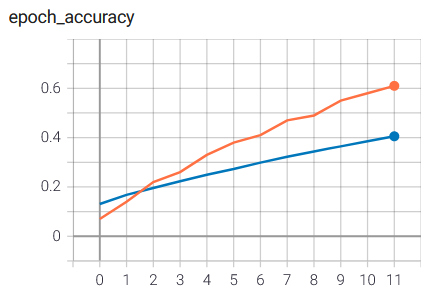
\includegraphics[width=0.49\textwidth]{TensorFlow/HistMNIST1acc}
		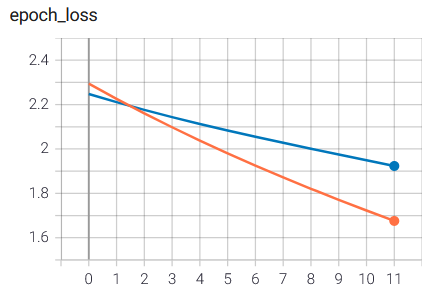
\includegraphics[width=0.49\textwidth]{TensorFlow/HistMNIST1loss}
		\caption{Trainingshistorie des einfachen Modells visualisiert mit TensorBoard} 
		\label{HistMNIST1}
	\end{center}
\end{figure}

\subsection{Probleme mit TensorBoard}

Bei der Verwendung von TensorBoard können Probleme bei dem Verbindungsaufbau, Laden der Daten oder Laden der \glqq richtigen\grqq{} Daten auftreten. Wenn zum Beispiel noch Daten angezeigt werden, die in der Zwischenzeit gelöscht wurden, oder aus einem anderen Grund ein komplettes Beenden und Neustarten des TensorBoards erzwungen werden soll, weil Tensorboard nicht mehr reagiert, können die folgenden Befehle - 
einzugeben im Windows command prompt - hilfreich sein:

\medskip


\SHELL{taskkill /im tensorboard.exe /f}

\SHELL{del /q \%TMP\%\textbackslash.tensorboard-info\textbackslash*}

\medskip

Es kann eine Fehlermeldung auftreten, dass die Datei nicht gefunden werden kann. Dies kann ignoriert werden. Nach kurzer Zeit sollte das TensorBoard dann neu geladen werden können.

\subsection{Neuronales Netz}

Um das neuronale Netz \glqq intelligenter\grqq  zu machen, wird eine zusätzliche, verdeckte Schicht, ein
sogenannter Hidden Layer, hinzugefügt. Diese Schicht besteht aus 200 Neuronen mit der ReLu-Aktivierungsfunktion. Eine weitere Verbesserung kann durch Dropout erzielt werden, die das Overfitting, also das Auswendiglernen der Trainingsdaten, vermeidet. Dies könnte auch durch eine wesentliche Erhöhung der Anzahl an Trainingsdaten erreicht werden, was aber natürlich auch eine wesentlich höhere Rechenzeit mit sich bringt. Stattdessen wird zwischen den beiden Schichten mit Neuronen eine Schicht eingefügt, die zufällig die Hälfte aller Informationen verwirft. Die neue Definition des Modells sieht wie folgt aus:

\begin{code}
    \begin{lstlisting}[numbers=none]
from tensorflow.keras.models import Sequential
from tensorflow.keras.layers import Dense,Flatten
from tensorflow.keras.layers import Dropout
model = Sequential()
model.add(Flatten())
model.add(Dense(200,activation='relu'))
model.add(Dropout(0.5))
model.add(Dense(10,activation='softmax'))
\end{lstlisting}

\caption{Neuronales Netz mit einer zweiten verdeckten Schicht und der Dropout-Funktion}
\end{code}

Wie in Abbildung~\ref{HistMNIST2} zu sehen ist, führt das Training mit dem neuronalen Netz und Dropout zu besseren Ergebnissen.

\begin{figure}[H]
	\begin{center}
		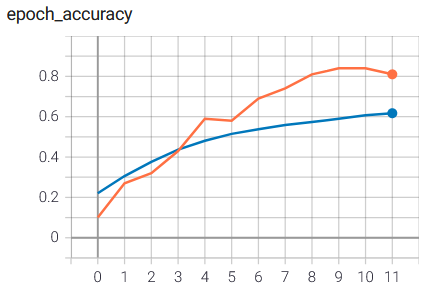
\includegraphics[width=0.49\textwidth]{TensorFlow/HistMNIST2acc}
		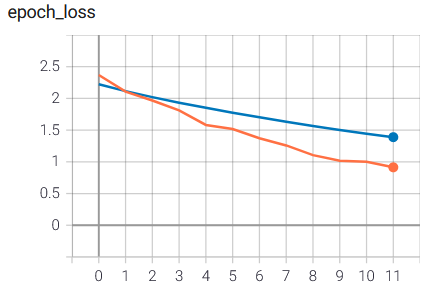
\includegraphics[width=0.49\textwidth]{TensorFlow/HistMNIST2loss}
		\caption{Trainingshistorie des einfachen Modells visualisiert mit TensorBoard} 
		\label{HistMNIST2}
	\end{center}
\end{figure}


\subsection{Convolutional Network}

%todo Quellen
Convolutional Networks eignen sich besonders für Aufgaben der Bildklassifizierung. Daher liegt der Gedanke natürlich nahe, sie auch hier zu verwenden. Dazu wird das Modell erneut neu definiert:

	
\begin{code}
    \begin{lstlisting}[numbers=none]
from tensorflow.keras.layers import Conv2D
from tensorflow.keras.layers import MaxPooling2D
model.add(Conv2D( 32, 
                  kernel_size=(3, 3),
                  activation='relu',
                  input_shape=input_shape))
model.add(Conv2D( 64, 
                  kernel_size=(3, 3),
                  activation='relu'))
model.add(MaxPooling2D(pool_size=(2, 2)))
model.add(Dropout(0.25))
model.add(Flatten())
model.add(Dense(200,
                activation = 'relu'))
model.add(Dropout(0.5))
model.add(Dense(10,
                activation = 'softmax'))
\end{lstlisting}
\caption{Aufbau eines Convolutional Netwerk}
\end{code}


\medskip

In diesem Modell sind nun zwei Faltungsschichten und eine Pooling-Schicht zu finden. Die neu hinzugefügten \PYTHON{Conv2D()}-Schichten gehören vor die bestehende Schicht \PYTHON{Flatten()}, da sie die zweidimensionale Struktur der Eingabebilder nutzen. Die erste Schicht lernt 32 Filter mit einer Matrixgröße von 3 $\times$ 3, die zweite 64 Filter. Darauf folgt eine Maximum-Pooling-Schicht, die jeweils nur den größten Wert von jedem $2 \times 2$-Feld speichert.

Mit dem auf 100 Samples begrenzten Trainingsdatensatz geht auch dieses Training noch schnell. Die Historie ist in Abbildung~\ref{HistMNIST3} abgebildet.

\begin{figure}[H]
	\begin{center}
		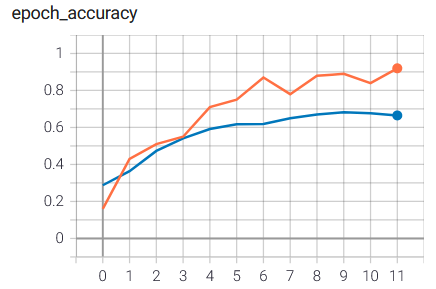
\includegraphics[width=0.49\textwidth]{TensorFlow/HistMNIST3acc}
		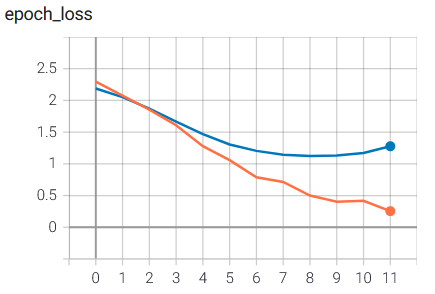
\includegraphics[width=0.49\textwidth]{TensorFlow/HistMNIST3loss}
		\caption{Trainingshistorie des einfachen Modells visualisiert mit TensorBoard} 
		\label{HistMNIST3}
	\end{center}
\end{figure}

Trainiert man über 12 Epochen mit allen 60.000 Trainingsdaten, dauert das Training auf einem Laptop mit AMD Ryzen 5 3500U Prozessor schon über 15 Minuten (ca. 1,5 Minuten je Epoche bei etwa 200ms pro Step). Dafür sind schon im sechsten Durchgang, Tensornboard zeigt dies als fünften an,  eine Genauigkeit von über 99 \% erreicht (siehe Abbildung~\ref{HistMNIST3_60000}).

\begin{figure}[H]
	\begin{center}
		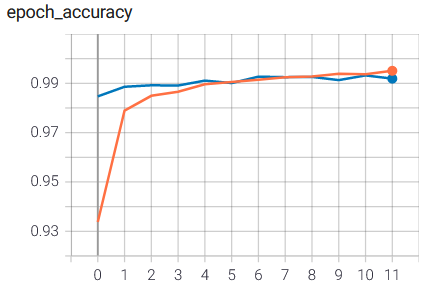
\includegraphics[width=0.49\textwidth]{TensorFlow/HistMNIST3acc_60000}
		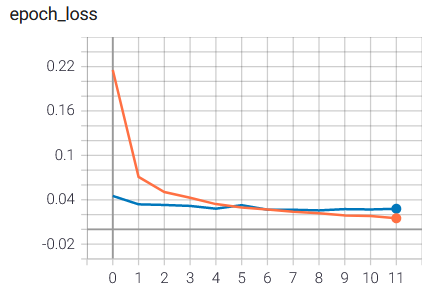
\includegraphics[width=0.49\textwidth]{TensorFlow/HistMNIST3loss_60000}
		\caption{Trainingshistorie des einfachen Modells visualisiert mit TensorBoard} 
		\label{HistMNIST3_60000}
	\end{center}
\end{figure}

\subsection{Vollständiger Code}

Der vollständige Code mit den zuvor beschriebenen Schritten und dem finalen CNN-Modell ist in Listing~\ref{TensorFlow:Complete} festgehalten. Er wurde mit Jupyter Notebook erstellt.

\begin{code}
\lstinputlisting[language=Python, firstnumber=1]{../Code/JetsonNano/MNIST.py}
%\includepdf[pages=-]{MNIST.pdf}
\caption{Erstellung eines Convolutional Netwerks}\label{TensorFlow:Complete}
\end{code}

%%%%%%%%%%%%%%%%%%%%%%%%%%%%%%%%%%%%%%%%%%%%%%%%%%%%%%%%%%%%        

\section{\glqq Hello World 2\grqq - Erkennung einer Iris}

Die Erkennung der Iris (Schwertlilie) ist ein weiterer Klassiker zur Bildklassifizierung. Auch zu diesem Klassiker gibt es mehrere Tutorials. \Mynote{Quellen} Die folgende Anleitung orientiert sich an dem Tutorial von \cite{KDnuggets.07.12.2020}.

Ziel dieses Tutorials ist die Klassifizierung dreier verschiedener Iris-Arten anhand vier verschiedener Attribute, der Länge und Breite des Kelchblatts (sepal) und des Blütenblatts (petal). Das heißt, der Ausgangspunkt ist eine Datei vom Format CSV. Allerdings liegen je Irisart nur 50 Messungen vor. Die Daten werden zu nächst durch die Verwendung eines \glqq OneHotVector\grqq{} normalisiert, so dass sie mit einem  neuronalen Netz verarbeitbar sind. Das verwendet neuronale Netz besteht aus neun verdeckten Schichten und einer Ausgabeschicht. Fünf verdeckte Schichten haben 64 Neuronen und vier haben 128. Für alle verdeckten Schichten wird die Aktivierungsfunktion ReLu verwendet. In der Ausgabeschicht ist die Aktivierungsfunktion SoftMax, so dass jeder Klasse ein Wahrscheinlichkeit zugeordnet wird. Es wird eine Genauigkeit von ungefähr 87 \% erreicht. Um ein Overfitting zu vermeiden wird schließlich noch mit einer Regularisierung gearbeitet.







\subsection{Laden der Daten Fisher's Iris Data Set}

Der Datensatz \glqq Iris\grqq{} wird mit der Bibliothek \PYTHON{sklearn} ausgeliefert.

\begin{code}
    \begin{lstlisting}[numbers=none]
from sklearn.datasets import load_iris
iris = load_iris()
\end{lstlisting}
\caption{Laden des Datensatzes Iris}
\end{code}

Für die Bilderkennung müssen wietere Bibliotheken geladen werden:

\begin{code}
    \begin{lstlisting}[numbers=none]
import numpy as np
import pandas as pd
import matplotlib.pyplot as plt

import tensorflow as tf
from tensorflow.keras.models import Sequential
from tensorflow.keras.layers import Dense
\end{lstlisting}
\caption{Bibliotheken für Hello World 2 - Iris}
\end{code}


Die Bibliotheken \FILE{numpy}, \FILE{pandas} und \FILE{pyplot} werden für die Vorbereitung und Visualisierung der Daten sowie der Darstellung der Ergebnisse verwendet. In einem neuronalen Netz werden die Berechnungen sequentiell abgearbeitet. Passend dazu wird der Modelltype \PYTHON{Sequential} importiert. Das Modell wird aus einzelnen Schichten aufgebaut, die sequentiell bearbeitet werden. Der Schichttyp \PYTHON{Dense} wird anschließend importiert. Der Schichttyp  ist eine Art von Schicht, die \glqq dicht\grqq{} verbunden ist, was bedeutet, dass alle Knoten der vorherigen Schicht mit allen Knoten der aktuellen Schicht verbunden sind.


Der Datensatz ist ein \PYTHON{dictionary}. Seine Schlüssel kann man sich leicht anzeigen lassen:

\medskip

\PYTHON{iris.keys()}

\medskip

als Output erhält man:

\medskip

\PYTHON{dict\_keys(['data', 'target', 'frame', 'target\_names', 'DESCR', 'feature\_names', 'filename'])}

\medskip

Die einzelnen Elemente kann man sich nun ansehen. Nach Eingabe des Befehls 

\medskip

\PYTHON{iris['DESCR']}

\medskip
wird eine ausführliche Beschreibung ausgegeben:

%'.. _iris_dataset:\n\nIris plants dataset\n--------------------\n\n**Data Set Characteristics:**\n\n    :Number of Instances: 150 (50 in each of three classes)\n    :Number of Attributes: 4 numeric, predictive attributes and the class\n    :Attribute Information:\n        - sepal length in cm\n        - sepal width in cm\n        - petal length in cm\n        - petal width in cm\n        - class:\n                - Iris-Setosa\n                - Iris-Versicolour\n                - Iris-Virginica\n                \n    :Summary Statistics:\n\n    ============== ==== ==== ======= ===== ====================\n                    Min  Max   Mean    SD   Class Correlation\n    ============== ==== ==== ======= ===== ====================\n    sepal length:   4.3  7.9   5.84   0.83    0.7826\n    sepal width:    2.0  4.4   3.05   0.43   -0.4194\n    petal length:   1.0  6.9   3.76   1.76    0.9490  (high!)\n    petal width:    0.1  2.5   1.20   0.76    0.9565  (high!)\n    ============== ==== ==== ======= ===== ====================\n\n    :Missing Attribute Values: None\n    :Class Distribution: 33.3% for each of 3 classes.\n    :Creator: R.A. Fisher\n    :Donor: Michael Marshall (MARSHALL%PLU@io.arc.nasa.gov)\n    :Date: July, 1988\n\nThe famous Iris database, first used by Sir R.A. Fisher. The dataset is taken\nfrom Fisher\'s paper. Note that it\'s the same as in R, but not as in the UCI\nMachine Learning Repository, which has two wrong data points.\n\nThis is perhaps the best known database to be found in the\npattern recognition literature.  Fisher\'s paper is a classic in the field and\nis referenced frequently to this day.  (See Duda & Hart, for example.)  The\ndata set contains 3 classes of 50 instances each, where each class refers to a\ntype of iris plant.  One class is linearly separable from the other 2; the\nlatter are NOT linearly separable from each other.\n\n.. topic:: References\n\n   - Fisher, R.A. "The use of multiple measurements in taxonomic problems"\n     Annual Eugenics, 7, Part II, 179-188 (1936); also in "Contributions to\n     Mathematical Statistics" (John Wiley, NY, 1950).\n   - Duda, R.O., & Hart, P.E. (1973) Pattern Classification and Scene Analysis.\n     (Q327.D83) John Wiley & Sons.  ISBN 0-471-22361-1.  See page 218.\n   - Dasarathy, B.V. (1980) "Nosing Around the Neighborhood: A New System\n     Structure and Classification Rule for Recognition in Partially Exposed\n     Environments".  IEEE Transactions on Pattern Analysis and Machine\n     Intelligence, Vol. PAMI-2, No. 1, 67-71.\n   - Gates, G.W. (1972) "The Reduced Nearest Neighbor Rule".  IEEE Transactions\n     on Information Theory, May 1972, 431-433.\n   - See also: 1988 MLC Proceedings, 54-64.  Cheeseman et al"s AUTOCLASS II\n     conceptual clustering system finds 3 classes in the data.\n   - Many, many more ...'

\begin{code}
\begin{lstlisting}[numbers=none]
'.. _iris_dataset:\n\nIris plants dataset
--------------------
**Data Set Characteristics:**
    :Number of Instances: 150 (50 in each of three classes)
   :Number of Attributes: 4 numeric, predictive attributes and the class
   :Attribute Information:
   - sepal length in cm
   - sepal width in cm
   - petal length in cm
   - petal width in cm
   - class:
            - Iris-Setosa
            - Iris-Versicolour
            - Iris-Virginica
            
   :Summary Statistics:
   ============== ==== ==== ======= =========================
   Min  Max   Mean    SD   Class Correlation
   ============== ==== ==== ======= ===== ====================
   sepal length:   4.3  7.9   5.84   0.83    0.7826
   sepal width:    2.0  4.4   3.05   0.43   -0.4194
   petal length:   1.0  6.9   3.76   1.76    0.9490  (high!)
   petal width:    0.1  2.5   1.20   0.76    0.9565  (high!)
   ============== ==== ==== ======= ===== ====================
       
   :Missing Attribute Values: None
   :Class Distribution: 33.3% for each of 3 classes.
   :Creator: R.A. Fisher
   :Donor: Michael Marshall (MARSHALL%PLU@io.arc.nasa.gov)
   :Date: July, 1988
       
   The famous Iris database, first used by Sir R.A. Fisher. The dataset is taken
   from Fisher\'s paper. Note that it\'s the same as in R, but not as in the UCI
   Machine Learning Repository, which has two wrong data points.
       
   This is perhaps the best known database to be found in the
   pattern recognition literature.  Fisher\'s paper is a classic in the field and
   is referenced frequently to this day.  (See Duda & Hart, for example.)  The
   data set contains 3 classes of 50 instances each, where each class refers to a
   type of iris plant.  One class is linearly separable from the other 2; the
   latter are NOT linearly separable from each other.
   .. topic:: References
   - Fisher, R.A. "The use of multiple measurements in taxonomic problems"
   Annual Eugenics, 7, Part II, 179-188 (1936); also in "Contributions to
   Mathematical Statistics" (John Wiley, NY, 1950).
   - Duda, R.O., & Hart, P.E. (1973) Pattern Classification and Scene Analysis.
     (Q327.D83) John Wiley & Sons.  ISBN 0-471-22361-1.  See page 218.
   - Dasarathy, B.V. (1980) "Nosing Around the Neighborhood: A New System
     Structure and Classification Rule for Recognition in Partially Exposed
     Environments".  IEEE Transactions on Pattern Analysis and Machine
     Intelligence, Vol. PAMI-2, No. 1, 67-71.
   - Gates, G.W. (1972) "The Reduced Nearest Neighbor Rule".  IEEE Transactions
     on Information Theory, May 1972, 431-433.
   - See also: 1988 MLC Proceedings, 54-64.  Cheeseman et al"s AUTOCLASS II
     conceptual clustering system finds 3 classes in the data.
   - Many, many more ...'
\end{lstlisting}
\caption{Informationen zum Datensatz Iris aus scikit-learn}
\end{code}


Mit der Eingabe

\medskip

\PYTHON{iris['feature\_names']}

\medskip

wird klar, dass die Eigenschaften, anhand derer die Blumen klassifiziert werden, die Länge und Breite des Kelchblatts (sepal) und Blütenblatts (petal) sind:



\begin{lstlisting}[numbers=none]
['sepal length (cm)',
 'sepal width (cm)',
 'petal length (cm)',
 'petal width (cm)']
\end{lstlisting}

Die Namen der Blumen, die nach der Eingabe

\medskip
\PYTHON{iris['target\_names']}

\medskip

angezeigt werden, sind

\begin{lstlisting}[numbers=none]
array(['setosa', 'versicolor', 'virginica'], dtype='<U10')
\end{lstlisting}

Zur weiteren Untersuchung werden die Daten mit den Überschriften in einen Datenrahmen aufgenommen.

\medskip

\PYTHON{x = pd.DataFrame(data = iris.data, columns = iris.feature\_names)}

\PYTHON{print(x.head())}

\medskip

Die Datenstruktur \PYTHON{x} enthält nur noch die ersten vier Spalten. Die Klasse wird später in den Datenstruktur \PYTHON{y} abgelegt. Diese Trennung musste zur Vorbereitung auf das Training erfolgen. Der Befehl \PYTHON{(x.head())} zeigt -- wie in Abbildung~\ref{TensorFlowHead} -- den Kopf des Datenrahmens an. Ersichtlich ist, dass jeder Datensatz aus vier Werten besteht. 

\begin{figure}[H]
	\GRAPHICSC{0.6}{1.0}{TensorFlow/IrisHead}
	\caption{Kopfzeilen des Datensatzes Iris}\label{TensorFlowHead}
\end{figure}

Jeder Datensatz enthält auch schon in dem Schlüssel \PYTHON{target} seine Klassifikation. In der Abbildung~\ref{TensorFlowHeadType} ist dies für die ersten Datensätze aufgeführt.

\medskip

\PYTHON{y = pd.DataFrame(data=iris.target, columns = ['irisType'])}

\PYTHON{y.head()}

\medskip

\begin{figure}[H]
	\GRAPHICSC{1.0}{1.0}{TensorFlow/IrisHeadType}
	\caption{Ausgabe der Kategorien des Datensatzes Iris}\label{TensorFlowHeadType}
\end{figure}

Mittels des Befehls 

\medskip

\SHELL{y.irisType.value\_counts()}

\medskip

kann ermittel werden, wie viele Klassen vorliegen. Die Ausgabe des Befehls wird in der Abbildung~\ref{TensorFlowIrisTypes} gezeigt; es ergeben sich 3 Klassen mit den Nummern $0$, $1$ und $2$. Jeweils 50 Datensätze sind ihnen zugeordnet.

\begin{figure}[H]
	\GRAPHICSC{1.0}{1.0}{TensorFlow/IrisTypes}
	\caption{Namen der Kategorien im Datensatz Iris}\label{TensorFlowIrisTypes}
\end{figure}


\subsection{Datenvorbereitung}

Nun kann der Prozess gestartet werden. Zunächst müssen die Daten vorbereitet werden.
In diesem Fall sind folgende Schritte notwendig: 

\begin{enumerate}
  \item Fehlende Werte müssen ergänzt werden.
  \item Die Daten müssen in Trainings- und Validierungsdaten aufgeteilt werden.
  \item Die Daten werden normalisiert.
  \item Die Daten, die Kategorien darstellen, müssen in einen Vektor umgewandelt werden.
  \item Die Daten werden in Vektoren eingetragen.
\end{enumerate}
	
\subsubsection{1. Fehlende Werte}

Mit dem Befehl 

\medskip

\PYTHON{pandas.DataFrame.info()}

\medskip

kann geprüft werden, ob die Daten konsistent sind. Die Abbildung~\ref{TensorFlowIrisInfo} zeigt, dass die Daten vollständig sind und der Datentype für alle Werte identisch ist. Demzufolge existiert für diesen Datensatz kein Handlungsbedarf.

\medskip

x.info()

\medskip

\begin{figure}[H]
	\GRAPHICSC{1.0}{1.0}{TensorFlow/IrisInfo}
	\caption{Prüfung des Datensatzes Iris}\label{TensorFlowIrisInfo}
\end{figure}


\subsubsection{2. Aufteilung in Trainigs- und Validierungsdaten}

Zur Aufteilung eines Datensatzes  in Trainings- und Validierungsdaten steht in der Bibliothek \PYTHON{sklearn} in der Klasse \PYTHON{model\_selection} die Methode \PYTHON{train\_test\_split} zur Verfügung. Hier werden 10\% des Datensatzes als Validierungsdaten zurückgehalten.

\medskip

\PYTHON{x\_train, x\_test, y\_train, y\_test = train\_test\_split(X,y, test\_size=0.1)}

\medskip

\subsubsection{3. Normalisierung der Daten}

Falls die Daten eine hohe Varianz haben, so sind sie zu normalisieren. Daher wird zuerst die Varianz ermittelt. Die Funktion \PYTHON{var()} steht dafür aus der Klasse \PYTHON{pandas.DataFrame} zur Verfügung. Die Ausgabe zeigt gemäß Abbildung~\ref{TensorFlowIrisVar}, dass die Varianz gering ist und somit kein Handlungsbedarf besteht.

\medskip

\PYTHON{x\_train.var(), x\_test.var()}

\medskip


\begin{figure}[H]
	\GRAPHICSC{1.0}{1.0}{TensorFlow/IrisVariance}
	\caption{Varianz im Datensatzes Iris}\label{TensorFlowIrisVar}
\end{figure}

\subsubsection{4. Konvertierung der Kategorien in einen Vektor}

Aus der Untersuchung des Datensatzes ist bekannt, dass drei Kategorien enthalten sind. Derzeit sind sie mit $0$, $1$ und $2$ nummeriert. Der verwendete Algorithmus könnte höhere Werte eine höhere Priorität zuordnen, so dass das Ergebnis verzerrt wird. Um dies zu vermeiden, wird ein Vektor generiert, der nur die
Wert $0$ und $1$ enthält und die Kategorie somit kodiert. Dies ist ein sogenannter \glqq OneHotVector\grqq{}. Dazu liegen zwei Möglichkeiten vor. Einmal könnte die Funktion \PYTHON{to\_categorical} der Bibliothek \PYTHON{Keras} verwendet werden oder die Funktion \PYTHON{OneHotEncoder} der Bibliothek \PYTHON{sklearn}.

\medskip

\PYTHON{y\_train = tf.keras.utils.to\_categorical(y\_train)}

\PYTHON{y\_test = tf.keras.utils.to\_categorical(y\_test)}

\medskip

Das Ergebnis der ersten fünf Daten zeigt die Abbildung~\ref{TensorFlowIrisCat} auf der rechten Seite. Es wird angezeigt mit

\medskip

\PYTHON{y\_train[:5,:]}

\medskip

Auf der linken Seite der Abbildung~\ref{TensorFlowIrisCat} ist die ursprüngliche Codierung der Kategorien angezeigt. Hier ist auch zu sehen, welche Datensätze zufällig als die ersten fünf
Trainingsdaten ausgewählt wurden.

\begin{figure}[H]
	\begin{center}
		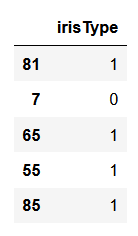
\includegraphics[width=0.2\textwidth]{TensorFlow/IrisCat1}
		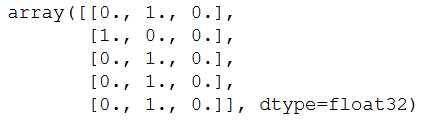
\includegraphics[width=0.6\textwidth]{TensorFlow/IrisCat}
		\caption{Codierung der Kategorien vor (links) und nach der Konvertierung} 
		\label{TensorFlowIrisCat}
	\end{center}
\end{figure}


\subsubsection{5. Konvertierung der Daten in Vektoren}

Damit die Daten einfacher weiterverarbeitet werden können, werden sie noch in Vektoren der Bibliothek \PYTHON{numpy} umgewandelt.

\medskip

\PYTHON{x\_train = x\_train.values}

\PYTHON{x\_test = x\_test.values}

\medskip


Das Ergebnis der Konvertierung kann im ersten Datensatz geprüft werden:

\medskip

\PYTHON{x\_train[0]}

\medskip
Das Ergebnis sieht wie folgt aus:

\begin{lstlisting}[numbers=none]
array([5.5, 2.4, 3.7, 1. ])
\end{lstlisting}


\subsection{Aufbau und Training des Modells}


Nach den Vorbereitungen kann nun das sequentielle Modell erstellt werden und die Schichten hinzugefügt werden.

\begin{code}
\begin{lstlisting}[numbers=none]
model1 = Sequential()
model1.add(Dense(64,activation='relu', input_shape= X_train[0].shape))
model1.add(Dense(128,activation='relu'))
model1.add(Dense(128,activation='relu'))
model1.add(Dense(128,activation='relu'))
model1.add(Dense(128,activation='relu'))
model1.add(Dense(64,activation='relu'))
model1.add(Dense(64,activation='relu'))
model1.add(Dense(64,activation='relu'))
model1.add(Dense(64,activation='relu'))
model1.add(Dense(3,activation='softmax'))
\end{lstlisting}

\caption{Aufbau des neuronalen Netzes für den Datensatz Iris}
\end{code}

In diesem Beispiel besteht das Model aus einer Eingabeschicht, acht versteckten Schichten und einer Ausgabeschicht. Die Aktivierungsfunktion der ersten Schichten ist die \PYTHON{relu}, nur für die Ausgabeschicht wird die Aktivierungsfunktion \PYTHON{softmax} verwendet, da diese den möglichen Kategorien Wahrscheinlichkeiten zuweist. Für den Fall, dass nur zwei mögliche Kategorien vorliegen, würde man die Aktivierungsfunktion \PYTHON{sigmoid} wählen. Neben der Aktivierungsfunktion \PYTHON{relu} stehen auch die Funktionen \PYTHON{sigmoid}, \PYTHON{linear} oder \PYTHON{tanh} zur Wahl. Die Experimente haben gezeigt, dass die Aktivierungsfunktion \PYTHON{relu} den besten Erfolg zeigt.

Die Eingabeschicht enthält ein zusätzliches Argument \PYTHON{input\_shape}. Dieses Argument sorgt, dafür, dass die Dimension der ersten Schicht sich an der Dimension eines Datensatzes orientiert. In diesem Beispiel ist die Größe vier.

Im nächsten Schritt wird nun das Modell fertiggestellt. Dazu muss der Optimierung, die Bewertungsfunktion und die Metrik übergeben werden.

\medskip

\PYTHON{model1.compile(optimizer='adam', loss= 'categorical\_crossentropy', metrics = ['acc'])}


\medskip

Für die Optimierungsfunktion stehen mehrere Kandidaten zur Verfügung:

\begin{itemize}
  \item \PYTHON{Stochastic Gradient Descent}, 
  \item \PYTHON{RMSProp} oder auch 
  \item \PYTHON{adam}.
\end{itemize}  

\medskip

 Hier wurde wie auch im vorherigen Beispiel \PYTHON{adam} verwendet.

Für die Bewertungsfunktion wird hier \PYTHON{categorical\_crossentropy} verwendet, die meistens in Klassifizierungsaufgaben mit mehreren Klassen verwendet wird, bei denen jeweils nur eine Kategorie richtig ist. Falls nur zwei Kategorien zur Verfügung stehen, so wird stattdessen \PYTHON{binary\_crossentropy} verwendet.

Metriken sind wichtig, um das eigene Modell zu bewerten. Es gibt verschiedene Metriken, anhand derer wir unser Modell bewerten können. Bei Klassifizierungsproblemen ist die wichtigste Metrik die Genauigkeit \PYTHON{['acc']}, die angibt, wie genau unsere Vorhersagen sind.

Im letzten Schritt wird das Modell nun anhand der Trainingsdaten trainiert.

\medskip

\PYTHON{history = model1.fit(x\_train, y\_train, batch\_size = 40, epochs=800, validation\_split = 0.1)}

\medskip

Für die Erstellung des Modells wurden hier 800 Epochen mit einer Batchgröße 40 eingestellt. Als Validierungsdaten werden zufällig 
10\% des Trainingsdatensatzes entnommen.

\subsection{Historie des Trainings und Visualisierung mit TensorBoard}

Die Methode \PYTHON{fit} gibt eine Datenstruktur zurück, die die gesamte Geschichte unseres Trainings enthält. So kann verfolgt werden, wie sich die Qualität während des Trainings entwickelt hat. Zum Beispiel kann durch wesentlich bessere Performance in den Trainingsdaten als in den Validierungsdaten ein Hinweis auf Overfitting entdeckt werden. Außerdem kann man sehen, ob die Qualität sich in den letzten Epochen asymptotisch verhält oder das Training verlängert werden sollte oder verkürzt werden kann.

Der Rückgabewert ist ein Dictionary, auf das mittels \PYTHON{history.history} zugegriffen werden kann.
 Hier kann man unter anderem  die Entwicklung der Genauigkeit im Trainings- als auch im Validierungsdatensatz
verfolgen. Auf die Historie der Elemente acc, loss, val\_loss und val\_acc können wir je mit history.history.loss oder history.history['val\_acc'] usw. zugreifen.


In der Abbildung~\ref{TensorFlowIrisPlotHist1} ist der Verlauf der Genauigkeit über die Epochen dargestellt. Für die Erzeugung des Graphen sind nur fünf Zeilen zu programmieren:

\medskip

\PYTHON{plt.plot(history.history['acc'])}

\PYTHON{plt.plot(history.history['val\_acc'])}

\PYTHON{plt.xlabel('Epochs')}

\PYTHON{plt.ylabel('Acc')}
    
\PYTHON{plt.legend(['Training', 'Validation'], loc='upper right')}

\medskip

\begin{figure}[H]
	\GRAPHICSC{0.8}{1.0}{TensorFlow/IrisPlotHist1}
	\caption{Verlauf der Genauigkeit für die Trainings- und Testdaten während des Trainings des Modells}\label{TensorFlowIrisPlotHist1}
\end{figure}

Analog kann der Verlauf der  Verlustfunktion gezeichnet werden:

\medskip

\PYTHON{plt.plot(history.history['loss'])}

\PYTHON{plt.plot(history.history['val\_loss'])}

\PYTHON{plt.xlabel('Epochs')}

\PYTHON{plt.ylabel('Loss')}

\PYTHON{plt.legend(['Training', 'Validation'], loc='upper left')}

\medskip

\begin{figure}[H]
	\GRAPHICSC{0.7}{1.0}{TensorFlow/IrisPlotHist2}
	\caption{Verlauf der Verlustfunktion für die Trainings- und Testedaten während des Trainings des Modells}\label{TensorFlowIrisPlotHist2}
\end{figure}

Laut \cite{KDnuggets.07.12.2020} erwarten wir, ein Overfitting zu beobachten, was sich darin äußert, dass die Ergebnisse für die Trainingsdaten deutlich besser sind als für die Validierungsdaten. In den erzielten Ergebnissen jedoch ist dieses Problem nicht zu erkennen. Die Validierungsdaten schneiden sogar besser ab als die Trainingsdaten. Vergleichen Sie dazu auch mit den Plots von \cite{KDnuggets.07.12.2020}. Eventuell wurden hier unterschiedliche Versionen von TensorFlow verwendet, die zu unterschiedlichen Ergebnissen führen.

Zur Überprüfung des Modells kann die Funktion  \PYTHON{model.evaluate} verwendet werden; die Methode erwartet die Testdaten mit den zugehörigen Kategorien:

\medskip

\PYTHON{model1.evaluate(x\_test, y\_test)}

\medskip

Die erreichte Genauigkeit auf die Testdaten liegt bei etwa 87 \%.

\subsection{Regularisierung}

Um ein besseres Modell zu erreichen, wird eine Regularisierung eingeführt. Dies reduziert die Gefahr des Overfittings, welches für das erste Modell erwartet wurde. In diesem Modell wird eine L2-Regularisierung hinzugefügt. Diese fügt in der Verlustfunktion zur Ermittlung der Gewichte den quadrierten Betrag des jeweiligen Koeffizienten als Strafterm hinzu.  

Als zweite Maßnahme zur Reduzierung des Overfittings und der Verbesserung des Modells, werden Dropout-Schichten hinzugefügt.

\begin{code}
    \begin{lstlisting}[numbers=none]
model2 = Sequential()
model2.add(Dense(64, activation = 'relu', input_shape= X_train[0].shape))
model2.add(Dense(128, activation = 'relu', kernel_regularizer=tf.keras.regularizers.l2(0.001)))
model2.add(Dense (128, activation = 'relu',kernel_regularizer=tf.keras.regularizers.l2(0.001)))
model2.add(tf.keras.layers.Dropout(0.5))
model2.add(Dense (128, activation = 'relu', kernel_regularizer=tf.keras.regularizers.l2(0.001)))
model2.add(Dense(128, activation = 'relu', kernel_regularizer = tf.keras.regularizers.l2(0.001)))
model2.add(Dense (64, activation = 'relu', kernel_regularizer=tf.keras.regularizers.l2(0.001)))
model2.add(Dense (64, activation = 'relu', kernel_regularizer=tf.keras.regularizers.l2(0.001)))
model2.add(tf.keras.layers.Dropout(0.5))
model2.add(Dense (64, activation = 'relu', kernel_regularizer=tf.keras.regularizers.l2(0.001)))
model2.add(Dense (64, activation = 'relu', kernel_regularizer=tf.keras.regularizers.l2(0.001)))
model2.add(Dense (3, activation = 'softmax', kernel_regularizer=tf.keras.regularizers.l2(0.001)))
\end{lstlisting}

\caption{Aufbau des neuronalen Netzes für den Datensatz Iris - Verbesserte Version}
\end{code}

Neben der Einführung der Regularisierung und der zwei Dropout-Schichten wird im Modell  und an den Parametern nichts geändert. 

\medskip

\begin{code}
    \begin{lstlisting}[numbers=none]
model2.compile(optimizer='adam', 
               loss='categorical_crossentropy', 
               metrics=['acc'])
history2 = model2.fit(x_train, y_train, 
                      epochs=800, 
                      validation_split=0.1, batch_size=40)
model2.evaluate(x\_test, y\_test)
\end{lstlisting}

\caption{Training des zweiten Modells}
\end{code}


\medskip

Auch für dieses Modell wird eine Genauigkeit von 87 \% anhand der Testdaten erreicht.

Den Verlauf der Genauigkeit und der Bewertungsfunktion werden in den Abbildungen \ref{TensorFlowIrisPlotHist3} und \ref{TensorFlowIrisPlotHist4} gezeigt. 


\begin{code}
    \begin{lstlisting}[numbers=none]
plt.plot(history2.history['acc'])
plt.plot(history2.history['val_acc'])
plt.title('Accuracy vs. epochs')
plt.ylabel('Acc')
plt.xlabel('Epoch')
plt.legend(['Training', 'Validation'], loc='lower right')
plt.show()
\end{lstlisting}

\caption{Verlauf der Genauigkeit und der Bewertungsfunktion}
\end{code}


\begin{figure}[H]
	\GRAPHICSC{0.8}{1.0}{TensorFlow/IrisPlotHist3}
	\caption{Verlauf der Genauigkeit für die Trainings- und Testdaten während des Trainings des zweiten Modells}
	\label{TensorFlowIrisPlotHist3}
\end{figure}


Der Python-Programmteil für die Verlustfunktion ist wie folgt gegeben:

\begin{code}
    \begin{lstlisting}[numbers=none]
plt.plot(history2.history['loss'])
plt.plot(history2.history['val_loss'])
plt.title('Loss vs. epochs')
plt.ylabel('Loss')
plt.xlabel('Epoch')
plt.legend(['Training', 'Validation'], loc='upper right')
plt.show()
\end{lstlisting}

\caption{Verlauf der Verlustfunktion}
\end{code}

\begin{figure}[H]
	\GRAPHICSC{0.8}{1.0}{TensorFlow/IrisPlotHist4}
	\caption{Verlauf der Verlustfunktion für die Trainings- und Testdaten während des Trainings des zweiten Modells}
	\label{TensorFlowIrisPlotHist4}
\end{figure}


\subsection{Vollständiger Code}

Das gesamte Skript des beschriebenen Tutorials findet sich in Listing~\ref{tensorflow:IrisComplete}.

\begin{code}
\lstinputlisting[language=Python, firstnumber=1]{../Code/JetsonNano/Iris.py}

\caption{Vollständiges Python-Programm für den Datensatz Iris}\label{tensorflow:IrisComplete}
\end{code}


